% This is based on the LLNCS.DEM the demonstration file of
% the LaTeX macro package from Springer-Verlag
% for Lecture Notes in Computer Science,
% version 2.4 for LaTeX2e as of 16. April 2010
%
% See http://www.springer.com/computer/lncs/lncs+authors?SGWID=0-40209-0-0-0
% for the full guidelines.
%
%
%     To submit at ISWC 2018 - Resource Track
%
%
\documentclass{llncs}

\hyphenation{do-cu-ment do-cu-ments}

\usepackage[utf8]{inputenc}

\usepackage{graphicx}
\usepackage{comment}
\usepackage{xspace}
\usepackage[usenames, dvipsnames]{xcolor}
\definecolor{igual}{rgb}{0.21, 0.11, 0} 
\usepackage{hyperref}
\definecolor{dark-blue}{rgb}{0.0,0.0,0.1}
\definecolor{dark-green}{rgb}{0.0,0.1,0.0}
\definecolor{dark-red}{rgb}{0.1,0.0,0.0}
\hypersetup{
    colorlinks, linkcolor={dark-red},
    citecolor={dark-green}, urlcolor={dark-blue},
    pdftitle={VoxEL: A Benchmark Dataset for Multilingual Entity Linking},    % title
    pdfauthor={Henry Rosales-Méndez, Barbara Poblete and Aidan Hogan},     % author
    pdfsubject={LD4IE 2017},   % subject of the document
    pdfkeywords={multilingual;} {entity linking;} {information extraction;}, % list of keywords
}
\usepackage{amsmath}
\newcommand{\argmin}{\arg\!\min}
\newcommand{\argmax}{\arg\!\max}

%para el simbolo de chequeado
\usepackage{amssymb}% http://ctan.org/pkg/amssymb
\usepackage{pifont}% http://ctan.org/pkg/pifont
\newcommand{\cmark}{\ding{51}}%
\newcommand{\xmark}{\ding{55}}%

\usepackage{booktabs} 
\usepackage{multirow}

\newcommand{\ah}[1]{{\color{blue}\textsc{ah:} #1}}

\usepackage{soul} %underline
\usepackage{pgfplots}
\begin{document}

\title{VoxEL: A Benchmark Dataset for \\Multilingual Entity Linking}
%
\titlerunning{}  % abbreviated title (for running head)
%                                     also used for the TOC unless
%                                     \toctitle is used
%
\author{Henry Rosales-M\'endez, Aidan Hogan and Barbara Poblete}
%
\authorrunning{Rosales-Méndez et al.} % abbreviated author list (for running head)
%
%%%% list of authors for the TOC (use if author list has to be modified)
%\tocauthor{Ivar Ekeland, Roger Temam, Jeffrey Dean, David Grove,
%Craig Chambers, Kim B. Bruce, and Elisa Bertino}
%
\institute{Millenium Institute for Foundational Research on Data\\Department of Computer Science, University of Chile \\
\texttt{\{hrosales,ahogan,bpoblete\}@dcc.uchile.cl}}

\newcommand{\ds}{\textsc{VoxEL}\xspace}

\maketitle              % typeset the title of the contribution
\begin{abstract}
%The Entity Linking (EL) task identify the entities mentions in a text corpus and associate them with corresponding entries in a knowledge base. Most EL approaches are suitable in the English context, but current trends are focused on agnostic-language approaches that allow us to perform EL over texts in many languages. One of the obstacles in multilingual contexts is that publicly available resources are scarce in multilingual contexts. This constitutes a hinder to achieve evaluation the quality of multilingual EL approaches, therefore, it is difficult to achieve progress in the area. In this work we propose VoxEL, a multilingual gold standard manually annotated that involve five languages that aim to favor the evaluation multilingual processes in EL. We also explore the behavior of state of the art of multilingual EL according to VoxEL and propose a new perspective to achieve multilingual annotations through automatic translation.

The Entity Linking (EL) task identifies entity mentions in a text corpus and associates them with corresponding entities in a given knowledge base. While traditional EL approaches have largely focused on English texts, current trends are towards language-agnostic or otherwise multilingual approaches that can perform EL over texts in many languages. One of the obstacles to ongoing research on multilingual EL is a scarcity of annotated datasets with the same text in different languages. In this work we thus propose \ds: a manually-annotated gold standard for multilingual EL featuring the same text expressed in five European languages. We first motivate and describe the \ds dataset. We then present the results of experiments using this dataset to compare the behavior of state of the art of (multilingual) EL systems across the five different languages, additionally comparing these results with methods using machine translation to English.
\keywords{Benchmark, Dataset, Multilingual Entity Linking}\\
\textbf{Resource type}: Dataset\\
\textbf{Permanent URL}: \url{https://dx.doi.org/10.6084/m9.figshare.6104759}
\end{abstract}

\section{Introduction} 
\label{sec:intro}

%There is a large amount of textual information available in an unstructured format, that is understandable to humans but difficult to process automatically by machine. 
%The vast amount of unstructured textual information available makes it impossible to assimilate for human beings, so automatic techniques are necessary to process it. In this context, Entity Linking (EL) is a task of Information Extraction (IE) that aim to bring some notion of \textcolor{red}{structure} in textual corpora, identifying and linking entities in the text with their corresponding knowledge-base entries. 

The Entity Linking (EL) task identifies entity mentions in a text corpus and associates them with corresponding entities in a Knowledge Base (KB). In this way, we can leverage the semantic information of publicly available KBs about real-world entities to achieve a better understanding of natural language text. For instance, in the text \textit{``in the world of pop music, there is Michael Jackson and there is everybody else''} quoted from The New York Times, we can link the mention \textit{Michael Jackson} with its corresponding entry in, for example, the Wikidata KB~\cite{Wikidata_vrandevcic2014wikidata} (\url{wd:Q2831}), or the DBpedia KB~\cite{dbpedia-lehmann2015dbpedia} (\url{dbr:Michael_Jackson})\footnote{Throughout, we use prefixes according to \url{http://prefix.cc}.} and thereafter leverage the knowledge in the KB about the entity mentioned in the text to support semantic search, relationship extraction, text enrichment, entity summarization, or semantic annotation, amongst other applications.

One of the major driving forces for research on EL has been the development of a variety of ever-expanding KBs that describe a broad selection of notable entities covering various domains (e.g., Wikipedia, DBpedia, Freebase, YAGO, Wikidata). Hence while traditional Named Entity Recognition (NER) tools focused on identifying mentions of entities of specific types in a text, EL further requires disambiguation of which entity in the KB is being spoken about; this remains a challenging problem. On the one hand, name variations -- such as \textit{``Michael Joseph Jackson''}, \textit{``Jackson''}, \textit{``The King of Pop''} -- mean that the same KB entity may be referred to in a variety of ways by a given text. On the other hand, ambiguity -- where the name \textit{``Michael Jackson''} may refer to various (other) KB entities, such as a journalist (\texttt{wd:Q167877}), a football player (\texttt{wd:Q6831558}), an actor (\texttt{wd:Q6831554}), and more besides -- means that an entity mention in a text may have several KB candidates associated with it.

%Another problem concerning to EL is the lack of consensus about the concept of ``entity''\cite{Borrega2007}. Some definitions of entity have been proposed in the literature by different areas of Natural Language Processes to response \textit{``what is an entity?''} but still remain an open issue~\cite{ourAMW2018}. As consequence, to decide when to select or not a mention for the annotation process is unclear in EL, as well as the inclusion or not of annotations in gold standards for evaluation purposes. In order to lessen this phenomenon Jha et al.~\cite{Jha2017} proposes a set of desirable properties that a gold standard must satisfy. On the other hand, \textcolor{red}{as we show in our previous work~\cite{ourAMW2018}}, we advocate for a more practical point of view inherent to EL that takes into account the domain of application rather a semantic perspective. Therefore, we encourage to answer better the question \textit{``what should Entity Linking link?''}. For Instance, coreferences are not so important if we want to find all documents about US singers, but relevant in extraction relation scenarios where many relations may be expressed in text with pronouns. \textcolor{red}{Two versions of this desirable behavior (relaxed and strict) would be fairer}. The popular EL system Babelfy\cite{Babelfy-moro2014entity} implements this criterion allowing us to specify if we only wish to annotate Proper Names, or include also concepts such as belt, bed, chair, table, etc.


Many research works have addressed these challenges of the EL task down through the years. Most of the early EL systems proposed in the literature were monolingual approaches focusing on texts written in one single language, in most cases English~\cite{mendes2011dbpedia,AIDA-hoffart2011robust}. These approaches often use resources of a specific language, such as Part-Of-Speech taggers and WordNet\footnote{\url{https://wordnet.princeton.edu}; April 1st, 2018}, that prevent generalization or adaptation to other languages. Furthermore, most of the labelled datasets available for training and evaluating EL approaches were English only (e.g., AIDA/CoNLL~\cite{aida2011}, DBpedia Spotlight Corpus\cite{mendes2011dbpedia}, KORE 50~\cite{kore50}). 

However, as the EL area has matured, more and more works have begun to focus on languages other than English, including multilingual approaches that are either language agnostic~\cite{THD-dojchinovski2012recognizing,daiber2013improving,ferragina2010tagme,mag2017} -- relying only on the language of labels available in the reference KB -- or can be configured for multiple languages~\cite{Babelfy-moro2014entity,freme-ner2016}. Recognising this trend, a number of multilingual datasets for EL were released, such as for the 2013 TAC KBP challenge\footnote{\url{https://tac.nist.gov/2013/KBP/}; April 1st, 2018} %, NTCIR\footnote{\url{http://ntcir.nii.ac.jp/CrossLink/}; April 1st, 2018} 
and the 2015 SemEval Task 13 challenge\footnote{\url{http://alt.qcri.org/semeval2015/task13/}; April 1st, 2018}. Although such resources are valuable for multilingual EL research -- where in previous work~\cite{Rosales-MendezP17} we presented an evaluation of EL systems comparing two languages from the SemEval dataset -- they have their limitations, key amongst which are their limited availability (participants only\footnote{We have managed to acquire the SemEval dataset, but unfortunately we were not able to acquire the TAC--KBP dataset: our correspondence was not responded to.}), a narrow selection of languages, and differences in text and annotations across languages that makes it difficult to compare performance across languages. More generally, the EL datasets available in multiple languages -- and languages other than English -- greatly lags behind what is available for English.

\paragraph{Contributions:} In this paper, we propose the \textsc{VoxEL} dataset: a manually-annotated gold standard for EL considering five European languages: German, English, Spanish, French and Italian languages. This dataset is based on an online source of multilingual news, where we select and annotate 15 corresponding news articles for these five languages (giving 45 articles in total). Additionally we create two versions of \textsc{VoxEL}: a \textit{strict} version where entities correspond to a restricted definition of entity as a mention of a person, place or organization (based on traditional MUC/NER definitions), and a \textit{relaxed} version where we consider a broader selection of mentions referring to entities described by Wikipedia. Based on the \textsc{VoxEL} dataset, using the GERBIL evaluation framework~\cite{gerbil-2015}, we present results for various EL systems, allowing us to draw comparisons not only across systems, but also across languages. As an additional contribution, we compare the performance of EL systems configurable for a given language with the analogous results produced by applying state-of-the-art machine translation (Google translate) to English and then applying EL configured for English.

\paragraph{Outline:} Section \ref{subsect:preliminaries} introduces preliminaries relating to the Entity Linking task. Section~\ref{sec:relatedWork} discusses works that have address the problem of multilingual Entity Linking, including discussion of both systems and datasets. Section~\ref{sec:voxel} presents the design and creation of the \textsc{VoxEL} dataset, along with some descriptive statistics. Section~\ref{sec:exp} presents some research questions that can be addressed with \textsc{VoxEL}, and presents corresponding experiments over a selection of EL systems. We then conclude and discuss future directions in Section~\ref{sec:conclusion}.


\section{Preliminaries}
\label{subsect:preliminaries}

We first introduce some preliminaries relating to EL. Let $E$ be a set of entity identifiers in a KB; these are typically IRIs, such as \texttt{wd:Q2831}, \texttt{dbr:Michael\_Jackson}. Given an input text, the EL process can be conceptualized in terms of two main phases. First, Entity Recognition (ER) establishes a set of entity mentions $M$, where each such mention is typically a string considered as referring to an entity, annotated with its start position in the input text, e.g., $(37,\textit{``Michael Jackon''})$. Second, for each mention $m\in{}M$ recognized by the first phase, Entity Disambiguation (ED) attepts to establish a link between $m$ and the corresponding identifier $e\in{}E$ for the KB entity to which it refers. The second disambiguation phase can be further broken down into a number of (typical) sub-tasks:

\begin{description}
\item \textit{Candidate entity generation}:
For each mention $m\in{}M$, this stage selects a subset of the most probable KB entities $E_m \subseteq E$ to which it may refer. There are two high-level approaches by which candidate entities are often generated. The first is a dictionary-based approach, which involves applying keyword or string matching between the mention $m$ and the label of entities from $E$. The second is an NER-based approach, where traditional NER tools are used to identify entity mentions (potentially) independently of the KB.

\item \textit{Candidate entity ranking}: This stage is where the final disambiguation is made: the candidate entities $E_m$ for each mention $m$ are ranked according to some measure indicating their likelihood of being the reference for $m$. The measures used for ranking each entity $e \in E_m$ may take into account features of the candidate entity $e$ (e.g., centrality), features of the candidate link $(m,e)$ (e.g., string similarity), features involving $e$ and candidates for neighbouring mentions $E_m'$ (e.g., graph distance in the KB), and so forth. Ranking may take the form of an explicit metric that potentially combines several measures, or may be implicit in the use of machine-learning methods that classify candidates, or that compute an optimal assignment of links.

\item \textit{Unlinkable mention prediction}: The target KBs considered by EL are often, by their nature, incomplete. In some applications, it may thus be useful to extract entity mentions from the input text that do not (yet) have a corresponding entity in the KB. These are sometimes referred to as \textit{emerging entities}, are typically produced by NER candidate generation (rather than a dictionary approach), and are assigned a label such as \textit{NIL} (Not In Lexicon). 
\end{description}

It is important to note that while the above processes provide a functional overview of the operation of most EL systems, not all EL systems follow this linear sequence of steps. Most systems perform recognition first, and once the mentions are identified the disambiguation phase is initiated~\cite{mendes2011dbpedia,Babelfy-moro2014entity}. However, other approaches may instead apply a unified process, building models that create feedback between the recognition and disambiguation steps~\cite{joinapproach2015}. In any case, the output of the EL process will be a set of links of the form $(m,e)$, where the mention $m$ in the text is linked to the entity $e$ in the KB, optionally annotated with a confidence score -- often called a \textit{support} --  for the link.


%===============================================================
\section{Related Work}
\label{sec:relatedWork}

We now cover related works in the context of multilingual EL, first discussing approaches and systems, thereafter discussing available datasets.

%-----------------------------------------------------------
\subsection{Multilingual EL Systems}
%.................
%% 1) HABLAR COSAS DE MULTILINGUAL
In theory, any EL system can be applied to any language; as we demonstrated in our previous work~\cite{Rosales-MendezP17}, even a system supporting only English components may still be able to correctly recognise and link the name of a person such as \textit{Michael Jackson} in the text of another language, assuming the alphabet remains the same. Hence the notion of a multilingual EL system can become blurred, where for example language-agnostic systems -- systems that require no linguistic components or resources specific to a language, typically ones based on a dictionary approach -- can become multilingual simply by virtue of having a reference KB with labels in a different -- or multiple different -- language(s). 

Here we thus focus on EL systems that have published evaluation results over texts from multiple languages, thus demonstrating proven multilingual capabilities. We summarise such systems in Table \ref{tab:multilingual_approaches}, where we provide details on the year of the main publication, the languages evaluated, as well as denoting whether or not a demo, source code or API is currently available.\footnote{We presented an earlier version of such a table in previous work~\cite{Rosales-MendezP17}.} As expected, a high-level inspection of the table shows that English is the most popularly-evaluated (and thus we surmise supported) language, followed by European languages such as German, Spanish, French, Dutch and Italian. We also highlight the year of publication, where -- with the exception of KIM \cite{KIM-popov2004kim} -- most of the included multilingual EL approaches have emerged since 2011.

\begin{table}[t]
	\centering
	\caption{Overview of multilingual EL approaches; the italicized approaches will be incorporated as part of our experiments}
	\label{tab:multilingual_approaches}
	\setlength{\tabcolsep}{3pt}
	\begin{tabular}{lccccr}
		\toprule
		\textbf{Name} &  \textbf{Year} & \textbf{Evaluated Languages} & \textbf{Demo} & \textbf{Src} & \textbf{API}\\ \midrule
		
		KIM \cite{KIM-popov2004kim} & 2004 &English, French, Spanish&\cmark&\xmark&\cmark\\\midrule
		
		SDA \cite{SDA-charton2011automatic}  & 2011 &English, French&\xmark&\xmark&\xmark\\\midrule
		
		ualberta \cite{guo2012ualberta}& 2012 &English, Chinese&\xmark&\xmark&\xmark\\\midrule
		
		HITS \cite{fahrni2012hits} & 2012 & English, Spanish, Chinese&\xmark&\xmark&\xmark\\\midrule
		
		\textit{THD} \cite{THD-dojchinovski2012recognizing}  & 2012 &English, German, Dutch&\cmark&\cmark&\cmark\\\midrule 
		
		\textit{DBpedia Spotlight} \cite{mendes2011dbpedia,daiber2013improving} & 2013  &English, Italian, Russian,&\cmark&\cmark&\cmark\\
		& &Dutch, French, German,&&&\\
		& &Spanish, Hungarian, Danish&&&\\\midrule
		
		\textit{TagME} \cite{ferragina2010tagme} & 2013 & English, German, Dutch &\cmark&\xmark&\cmark\\\midrule
		
		Wang-Tang \cite{wang2013boosting} & 2013 & English, Chinese&\xmark&\xmark&\xmark\\\midrule
		
		\textit{AGDISTIS} \cite{usbeck2014agdistis,mag2017}& 2014 & English, German, Spanish&\cmark&\cmark&\cmark\\
		& &French, Italian, Japanese,&&&\\
		& &Dutch&&&\\\midrule
		
		\textit{Babelfy} \cite{Babelfy-moro2014entity}& 2014 &English, Spanish, French &\cmark&\xmark&\cmark\\
		& &German, Italian&&&\\\midrule
		
		\textit{FREME}~\cite{freme-ner2016}&2016&English, German&\xmark&\cmark&\cmark\\\midrule
		%& &French, Spanish, Russian&&&\\\midrule
		
		WikiME \cite{Cross-Lingual-Wikifier-tsai2016cross} & 2016 & English, Spanish, French,&\cmark&\xmark&\xmark\\
		& &Italian, Chinese, German,&&&\\
		& &Thai, Arabic, Turkish,&&&\\
		& &Tamil, Tagalog, Urdu, Hebrew&&&\\\midrule		
		
		FEL~\cite{FEL-pappu2017lightweight}& 2017 &English, Spanish, Chinese&\xmark&\cmark&\xmark\\\midrule
		
		FOX~\cite{fox2017}&2017&English, German, Spanish,&\cmark&\cmark&\cmark\\
		& & French, Dutch &&&\\
		
		%&2016&IDIOMAS&\cmark&\cmark&\cmark\\
		%& & French, Dutch &&&\\
		\bottomrule
	\end{tabular}
\end{table}

We will later conduct experiments using the GERBIL evaluation framework~\cite{GERBIL_usbeck2015evaluating}, which allows for invoking and integrating the results of a variety of public APIs for EL, generating results according to standard metrics in a consistent manner. Hence, in our later experiments, we shall only consider those systems with a working REST-API made available by the authors of the system. In addition, we will manually label our \textsc{VoxEL} system according to Wikipedia, with which other important KBs such as DBpedia, YAGO, Freebase, Wikidata, etc., can be linked; hence we only include systems that support such a KB linked with Wikipedia. With these criteria in mind, we select the following systems: 

\begin{description}
\item[THD (2012)] is based on three measures~\cite{THD-dojchinovski2012recognizing}: \textit{most frequent senses}, which ranks candidates for a mention based on the Wikipedia Search API results for that mention; \textit{co-occurrence}, which is a co-citation measure looking at how often candidate entities for different mentions are linked from the same paragraphs in Wikipedia; and \textit{explicit semantic analysis}, which uses keyword similarity measures to relate mentions with a concept. These methods are language agnostic and applicable to different language versions of Wikipedia.
\item[DBpedia Spotlight (2013)] was first proposed to deal with English annotations~\cite{mendes2011dbpedia}, based on keyword and string matching functions ranked by a probabilistic model based on a variant of a TF--IDF measure. DBpedia Spotlight is largely language-agnostic, where an extended version later proposed by Daiber et al.~\cite{daiber2013improving} leverages the multilingual information of the Wikipedia and DBpedia KBs to support multiple languages.
\item[TagMe (2013)] uses analyses of anchor texts in Wikipedia pages to perform EL~\cite{ferragina2010tagme}. The ranking stage is based primarily on two measures: \textit{commonness}, which describes how often an anchor text is associated with a particular Wikipedia entity; and \textit{relatedness}, which is a co-citation measure indicating how frequently candidate entities for different mentions are linked from the same Wikipedia article. TagMe is language agnostic: it can take advantage of the Wikipedia Search API to apply the same conceptual process over different language versions of Wikipedia to support multilingual EL.
\item[AGDISTIS (2014)] assumes that recognition has been performed using another tool and thus, given a set of mentions, focuses on the disambiguation process~\cite{usbeck2014agdistis}. The generation of candidates is mainly performed over indexes computed off-line from the target KB, where the ranking stage computes an assignment of links from related entities in a graph built over neighbouring candidate entities and mentions. A recent study \cite{mag2017} extends this approach, adding some new features to improve its behavior in multilingual scenarios. 
\item[Babelfy (2014)] performs EL with respect to a custom multilingual KB BabelNet~\footnote{\url{http://babelnet.org/}; April 1st, 2018} constructed from Wikipedia and WordNet, using machine translation to bridge the gaps in information available for different language versions of Wikipedia~\cite{Babelfy-moro2014entity}. Recognition is based on POS tagging for different languages, selecting candidate entities by string matching. Ranking is reduced to finding the densest subgraph that relates neighbouring entities and mentions.
\item[FREME (2016)] delegates the recognition of entities to the Stanford-NER tool, which is trained over the anchor texts of Wikipedia corpora in different languages. Candidate entities are generated by keyword search over local indexes, which are then ranked based on the number of matching anchor texts in Wikipedia linking to the corresponding article of the candidate entity~\cite{freme-ner2016}.
\end{description}

\ah{Any explanation for not including FOX?}





\subsection{Multilingual EL Datasets}
%.................
%3) HABLAR SOBRE LOS corpus actuales monolingues

In order to train and evaluate EL approaches, labelled datasets -- annotated with the correct entity mentions and their respective KB links -- are essential. In some cases these datasets are labelled manually, while in other cases labels can be derived from existing information, such as anchor texts. In Table \ref{tab:datasets} we survey the labelled datasets most frequently used by EL approaches (note that sentence counts were not available for some datasets).

\newcommand{\ccell}[1]{\multicolumn{1}{c}{#1}}
\setlength{\tabcolsep}{1.2ex}
\begin{table}[tb!]
\centering

\caption{Survey of dataset for EL task. For multilingual datasets, the quantities shown refer to the English data available. We present metadata about the relaxed and strict version of our dataset by VoxEL$_R$ and VoxEL$_S$ respectively. (Abbreviations: $|D|$ number of documents, $|S|$ number of sentences, $|E|$ number of entities, \textbf{Mn} denotes that all entities were manually annotated.)}
\label{tab:datasets} 
\begin{tabular}{lrrrcc}
\toprule
\textbf{Dataset}~~~~~~~~~~~~~~~~~~ & \ccell{$|D|$} & \ccell{$|S|$} & \ccell{$|E|$} & \ccell{\textbf{Mn}} & \ccell{\textbf{Languages}}\\\midrule
AIDA/CoNLL-Complete~\cite{aida2011} &1393    &22,137 &34,929  &\cmark  &EN \\\midrule
AIDA/CoNLL-Test A~\cite{aida2011}   &216     &3,466  &5,917   &\cmark  &EN \\\midrule
AIDA/CoNLL-Test B~\cite{aida2011}   &231     &3,684  &5,616   &\cmark  &EN \\\midrule
AIDA/CoNLL-Training~\cite{aida2011} &946     &14,987 &23,396  &\cmark  &EN \\\midrule
KORE50~\cite{kore50}                &50      &50     &144     &\cmark  &EN \\\midrule
IITB~\cite{IITB2009}                &103     &1,781  &18,308  &\cmark &EN \\\midrule
ACE2004~\cite{ace04}                &57      &-      &306     &\xmark &EN\\\midrule
%OKE challenge 2016                 &\xmark  &\cmark &\cmark  & &\xmark \\\midrule
AQUAINT~\cite{aquaint}              &50      &533    &727     &\xmark &EN \\\midrule
MSNBC~\cite{MSNBC07}                &20      &668    &747     &\xmark &EN \\\midrule
DBpedia Spotlight
\cite{mendes2011dbpedia}            &10      &58     &331     &\cmark &EN \\\midrule
N3-RSS 500~\cite{n3}                &1       &500    &1000    &\cmark  &EN \\\midrule
Reuters 128~\cite{n3}               &128     & -     &881     &\cmark  &EN \\\midrule
Wes2015~\cite{wes2015}              &331     & -     &28,586  &\cmark  & EN \\\midrule
%Derczynski                         &\xmark  &\xmark &\cmark  & &\cmark \\\midrule
News-100~\cite{n3}                  &100     &-      &1656    &\cmark  &DE \\\midrule
Thibaudet~\cite{renden2016}         &1       &3,807  &2,980   &\xmark  &FR \\\midrule
Bergson~\cite{renden2016}           &1       &4,280  &380     &\xmark  &FR \\\midrule
SemEval 2015 
Task 13~\cite{moro2015semeval}      &4       &137    &769     &\cmark &EN,ES,IT \\ \midrule
DBpedia Abstracts
~\cite{abstracts2016}               &39,132  &-      &505,033 &\xmark &DE,EN,ES,FR, \\
                                    &        &       &        &       &IT,JA,NL \\\midrule
MEANTIME \cite{meantime2016}        &120     &597    &2,790   &\xmark &EN,ES,IT,NL \\\midrule 
VoxEL$_R$                           &15      &94     &674     &\cmark &DE,EN,ES,FR,IT\\\midrule  
VoxEL$_S$                           &15      &94     &204     &\cmark &DE,EN,ES,FR,IT\\ 
\bottomrule
\end{tabular}
\end{table}

We can see that the majority of datasets provide text in one language only -- predominantly English -- with the exceptions being as follows: 

\begin{description}
\item[SemEval 2015 Task 13:] is built over a biomedical, math, computer and social domain and is designed to support EL and WSD at the same time, containing annotations to Wikipedia, BabelNet and WordNet~\cite{moro2015semeval}.
\item[DBpedia Abstracts:] provides a large-scale training and evaluation corpora based on the anchor texts extracted from the abstracts (first paragraph) of Wikipedia pages in seven languages \cite{abstracts2016}.\footnote{\url{http://wiki-link.nlp2rdf.org/abstracts/}; April 1st, 2018} 
\item[MEANTIME:] consists of 120 news articles from WikiNews\footnote{\url{https://en.wikinews.org/}; April 1st, 2018} with manual annotations of entities, events, temporal information and semantic roles \cite{meantime2016}.\footnote{\url{http://www.newsreader-project.eu/results/data/wikinews/}; April 1st, 2018} 
\end{description}

Amongst these multilingual datasets, we can highlight a number of shortcomings. First note that we do not include the 2013 TAC--KBP dataset in this list since it was not available at the time of writing. 

With respect to DBpedia Abstracts, while offering a very large multilingual corpus, the texts across different languages varies, as do the documents available; while such a dataset could be used to compare different systems for the same languages, it could not be used to compare the same systems for different languages. Furthermore, there are no guarantees possible for the completeness of the annotations since they are anchor texts/links extracted from Wikipedia; hence the dataset is best suited as a (very) large collection of positive examples -- in a similar manner to how TagMe~\cite{ferragina2010tagme} and FREME~\cite{freme-ner2016} use anchor texts -- rather than an evaluation dataset since it cannot reliably identify false positives.

Unlike DBpedia Abstracts, the SemEval and MEANTIME datasets contain analogous documents translated to different languages. However, MEANTIME and SemEval 2015 Task 13 uses machine translation from English to obtain the text in the other languages. Despite the tremendous progress made in machine translation in recent years, translation errors are still a possibility, particularly where entity labels are involved. For example, while Google Translate would currently translate the Spanish sentence ``\textit{Vi la película {\scriptsize$\ll$}Jungla de cristal{\scriptsize$\gg$ }ayer.}'' to ``\textit{I saw the movie `Crystal Jungle' yesterday.}'', a human expert would rather translate it as ``\textit{I saw the movie `Die Hard' yesterday.}''. In previous work we conducted a comparison of EL systems for English and Spanish texts using the SemEval dataset; we refer the reader to~\cite{Rosales-MendezP17} for more details, including results.

%Involving more than one language is differently implemented by KBs. While Wikipedia separates the entities by languages, structured KBs such as Wikidata gather in the same multilingual resource all the information about each entity for all the languages supported. %BabelNet constitute other multilingual KB that follows this desirable property, constructed over Wikipedia but without the information conflict problems of it. The gap between the different editions of Wikipedia was filled in BabelNet mainly with automatic translation. 
%Having information gathered in this way allow EL systems to use the same link to annotate the same mentions in different languages, but in an environment like Wikipedia there are two ways make the annotations. For a given text input written in a specific language $L$, either the approaches target the entities of the version of the language $L$ of the KB (e.g., DBpedia Spotlight, AGDISTIS), or target the English version of the KB whatever the language $L$ is.%\textcolor{red}{We refer to the second ways of annotation in this paper as \textit{cross-lingual} links (e.g., Tagme, Babelfy).}

%However, MEANTIME and SemEval 2015 Task 13 use the automatic translation from English to obtain the text in the other languages. Despite the tremendous progress made in automatic translation in the last years, it can happen that it introduces translation errors. In this context, approaches based on grammar or any linguistic information could be devalued. 

%TOur dataset VoxEL is built over curted achiving the annotation through five languages.



%===========================================================================
\section{The VoxEL Dataset} \label{sec:voxel}

In this section, we describe the \textsc{VoxEL} Dataset that we propose as a gold standard for EL involving five languages: German, English, Spanish, French and Italian. \textsc{VoxEL} is based on 15 news articles sourced from the VoxEurop\footnote{\url{http://www.voxeurop.eu/}; April 1st, 2018} web-site: a European newsletter with the same news articles professionally translated to different languages. This source of text thus obviates the need for translation of texts to different languages, and facilitates the consistent identification and annotation of mentions (and their Wikipedia links) across languages. With VoxEL, we thus provide a high-quality resource with which to evaluate the behavior of EL systems across a variety of European languages. 

While the VoxEurop newsletter is a valuable source of professionally translated text in several European languages, there are sometimes natural variations across languages that -- although they preserve meaning -- may change how the entities are mentioned. A common example is the use of pronouns rather than repeating a person's name to make the text more readable in a given language. Such variations would then lead to different entity annotations across languages, hindering comparability. Hence, in order to achieve the same number of sentences and annotations for each new (document), we applied small manual edits to homogenize the text (e.g., replacing a pronoun by a person's name). On the other hand, sentences that introduce new entities in one particular language, or that deviate too significantly across all languages, are eliminated.

With respect to the guidelines for labelled entity mentions, we take into consideration the lack of consensus about what is an ``\textit{entity}'': some works conservatively consider only mentions of entities referring to fixed types such as person, organization and location as entities (similiar to the traditional NER/TAC consensus on an entity) \ah{refs from AMW paper}, while other authors note that a much more diverse set of entities are available in Wikipedia and related KBs for linking, and thus consider any noun-phrase mentioning an entity in Wikipedia to be a valid target for linking \ah{refs from AMW paper}. Furthermore, there is a lack of consensus on how overlapping entities -- like \textit{New York City Fire Department} -- should be treated \ah{ref from AMW}; should \textit{New York City} be annotated as a separate entity or should we only cover maximal entities? Rather than take a stance on such questions -- which appear application dependant -- we instead create two versions of the data: a \textit{strict} version that considers only maximal entity mentions referring to persons, organizations and locations; and a \textit{relaxed} version that considers any noun phrase mentioning a Wikipedia entity as a mention, including overlapping mentions where applicable.

\ah{Henry: could you add an example strict and relaxed sentence in English for comparison? Something relatively clean?}

%Taking into consideration the lack of consensus about \textit{``what is an entity?''} we propose handle two points of view of the annotations for the same input text. First, a \textit{relaxed} version that includes any Wikipedia page that is not disambiguation or redirection. Second, a \textit{strict} version that points only to irrefutable Wikipedia entities, and that are person, organization or place. Thus we can measure the behavior of systems according to its application domain. Some systems have a general purpose and allow us to adapt to the application domain, for instance, DBpedia Spotlight allow us to specify the confidence and support parameters with use to decide which entity links. Although these two parameters allow adjustment to the context, they should be calibrated each time it changes. An idea closer to our objective is the behavior of Babelfy, which allows us to specify if we want to annotate only entities, or if we allow the inclusion of concepts.

To create the annotation of mentions with corresponding KB identifiers, we implemented a Web tool\footnote{\url{https://users.dcc.uchile.cl/~hrosales/NIFify.html}} that allows a user annotate a text, producing output in the popular NLP Interchange Format (NIF)~\cite{nif2013}, as well as offering visualizations of the annotations that facilitate, e.g., revision. For each language, we provide annotated links that target the English Wikipedia entry, as well the language version of Wikipedia (if different from English). In case there was no appropriate Wikipedia entry for a mention of a person, organization or place, we annotate the mention with a \url{NotInLexicon} marker.

In summary, \textsc{VoxEL} thus consists of 15 news (documents) from the multilingual newsletter VoxEurop, totalling 94 sentences. This text is annotated times five for each language, and times two for the strict and relaxed versions, giving a total of 150 annotated documents and 940 sentences. The same number of annotations is given for each language (including by sentence). For the strict version, each language has 204 annotated mentions, while for the relaxed version, each language has 674 annotated mentions. Again, this homogeneity of text and annotations across languages was non-trivial to achieve, but facilitates comparison of evaluation results not only across systems, but across languages. For comparison, the SemEval dataset has 758, 768 and 784 annotations in the English, Spanish and Italian version respectively, while MEANTIME has 2790, 2729, 2709 and 2704 mentions in the English, Dutch, Italian and Spanish versions of their text.

%============================================================================
\section{Experiments}\label{sec:exp}

We now use our proposed VoxEL dataset to conduct experiments in order to explore the behavior of state of the art EL systems for multilingual settings. In particular, we are interested in the following questions:

\begin{itemize}
\item \textbf{RQ1}: How does EL performance of state-of-the-art systems differ for the German, English, Spanish, French and Italian languages? 
\item \textbf{RQ2}: Could automatic translation be used to achieve results similar to that achieved in the English language by monolingual systems applied to texts written in a language that does not have its configuration?
\item \textbf{RQ3}: Taking into account that the systems obtain a better performance for English, could the automatic translation overcome the results of such systems for the other languages that support VoxEL?.
\end{itemize}

To response RQ1 we ran the multilingual systems Babelfy, AGDISTIS, DBpedia Spotlight, FREME NER, TagME and THD over both version of VoxEL. The results are shown in Table~\ref{tab:gerbil}. We use these systems via their REST APIs maintaining its predetermined parameters, except for the case of Babelfy for which we analyze separately the inclusion (Babelfy$_r$) and not inclusion (Bablfy$_s$) of concepts in the annotations. This first experiment was conducted by designing a modified local version of GERBIL~\cite{gerbil2015}, which is a friendly platform with a suits of annotator and datasets available for agile comparisons. So far, GERBIL only consider English comparison, therefore, we include missing configurations in order that multilingual systems could annotate non-English texts. 


\begin{table}[tb!]
\centering
\caption{Evaluation of EL systems according GERBIL using Micro F$_1$. We refer FREME NER and DBpedia Spotlight as \textit{FREME} and \textit{DBspot} respectively. In the cases when no result was obtained we show $err$, as well as ``-'' when a system does not support the corresponding language.}
\label{tab:gerbil}
\resizebox{\textwidth}{!}{
	\begin{tabular}{@{}lcccccccccccc@{}}
%\begin{tabular}{@{}lllllllllll@{}}
\toprule
            && \multicolumn{5}{c}{Relax}   & \multicolumn{5}{c}{Strict}  \\ \midrule
            &&~~DE~~~&~~EN~~~&~~ES~~~&~~FR~~~&~~IT~~~&~~DE~~~&~~EN~~~&~~ES~~~&~~FR~~~&~~IT~~~\\
            \cmidrule(lr){3-7}\cmidrule(lr){8-12}
            &$mP$& 0,840& 0.649 & 0.835 & 0.824 & 0.810 & 0.932 & 0.785 & 0.929 & 0.889 & 0.907 \\
Babelfy$_r$ &$mR$& 0.181& 0.522 & 0.549 & 0.488 & 0.451 & 0.676 & 0.735 & 0.710 & 0.632 & 0.578 \\
            &$mF$& 0.595& 0.578 & 0.662 & 0.613 & 0.579 & 0.784 & 0.759 & 0.805 & 0.739 & 0.706 \\\midrule
            &$mP$& 0.903& 0.722 & 0.916 & 0.912 & 0.884 & 0.942 & 0.816 & 0.923 & 0.912 & 0.894 \\
Babelfy$_s$ &$mR$& 0.461& 0.219 & 0.210 & 0.200 & 0,192 & 0.558 & 0.524 & 0.593 & 0.563 & 0.583 \\
            &$mF$& 0.301& 0.336 & 0.342 & 0.328 & 0.316 & 0.701 & 0.638 & 0.722 & 0.697 & 0.706 \\\midrule
            &$mP$& 0.313& 0.348 & 0.437 & 0,282 & 0.512 & 0.568 & 0.779 & 0.549 & 0.475 & 0.725 \\
AGDISTIS    &$mR$& 0.237& 0.265 & 0.329 & 0,210 & 0,397 & 0.568 & 0.779 & 0.549 & 0.475 & 0.725 \\
            &$mF$& 0.270& 0.301 & 0.376 & 0.241 & 0.447 & 0.568 & 0.779 & 0.549 & 0.475 & 0.725 \\\midrule
            &$mP$& 0.731& 0.745 & 0.691 & 0.658 & 0.682 & 0.781 & 0,854 & 0.690 & 0.691 & 0.800  \\
DBspot      &$mR$& 0.508& 0.577 & 0.399 & 0.360 & 0.488 & 0.544 & 0.602 & 0.382 & 0.406 & 0.549  \\
            &$mF$& 0.600& 0.650 & 0.506 & 0.466 & 0.569 & 0.641 & 0.706 & 0.492 & 0.512 & 0.651 \\\midrule
            &$mP$& $err$& 0.781 & $err$ & $err$ & $err$ & $err$ & 0.872 & $err$ & $err$ & $err$  \\
FREME       &$mR$& $err$& 0.370 & $err$ & $err$ & $err$ & $err$ & 0.402 & $err$ & $err$ & $err$  \\
            &$mF$& $err$& 0.503 & $err$ & $err$ & $err$ & $err$ & 0.550 & $err$ & $err$ & $err$ \\\midrule
            &$mP$& 0.635& 0.754 & -     & -     & 0.494 & 0.875 & 0.946 & -     & -     & 0.742  \\
TagME       &$mR$& 0.232& 0.488 & -     & -     & 0.182 & 0.652 & 0.784 & -     & -     & 0.509  \\
            &$mF$& 0.340& 0.592 & -     & -     & 0.266 & 0.747 & 0.857 & -     & -     & 0.604 \\\midrule
            &$mP$& 0.831& 0.806 & -     & -     & -     & 0.857 & 0.809 & -     & -     & -     \\
THD         &$mR$& 0.109& 0.253 & -     & -     & -     & 0.352 & 0.647 & -     & -     & -     \\
            &$mF$& 0.194& 0.386 & -     & -     & -     & 0.500 & 0.719 & -     & -     & -    \\\bottomrule 
\end{tabular}
}
\end{table}

We show in Table~\ref{tab:gerbil} the Micro F$_1$ obtained in the experiment\footnote{The GERBIL results are available at \url{https://users.dcc.uchile.cl/~hrosales/ISWC2018_experiment_GERBIL.html}}. While DBpedia Spotlight and FREME NER show a similar behavior in both environment, Babelfy, AGDISTIS, TagME and THD are sensitives to the inclusion of entities that do not are persons, organizations or places. In all of the cases, the involved systems agree with the fact that the strict version of VoxEL better fits the task needs. 

Incorporating more than one language into an EL approach brings with it an increase in its complexity. For instance, WikiME uses a model based on word embedding, which includes a final step for each foreign language embeddings of projection to the English one. On the other hand, Babelfy exploits the sets of synonyms of BabelNet\footnote{\url{http://babelnet.org/} KB; April 1st, 2018}, called \textit{Babel synsets}, that groups words in different languages to achieve multilingual EL. According to our review, no system has used machine translation to address the language barriers in EL. Some work with automatic translation is done in related areas, such as cross-lingual ontology matching~\cite{fu2010} where the impact of the translation quality is stressed.

In this direction, we design a second experiment in order to study the behavior of these same approaches configured only for English over the non-English version of VoxEL by automatic translation to English. For the automatic translation we use Google translator\footnote{\url{https://translate.google.com/}; April 1st, 2018}. VoxEL contains links to the language for each of its versions and also to English, what makes it possible to evaluate automatic translations directly. However, when we apply the translation we lost the details of the annotation information that it is required by GERBIL, such as the translated mention, initial and final position of the mention, etc. For this reason, we implement our own benchmark that leaves out the mentions information of the evaluation process, only considering the match between the URIs of the gold standard and the system results. 

In Table \ref{tab:translations} we show the results of the second experiment, showing the MicroF$_1$ score obtained for each system over the version of VoxEL written in its five languages. We configure the system with English and ran then over the version of VoxEL in the original language $L$ and also in the translated version, with the aim of having a point of reference that allows to mediate a worse and better behavior of the system on VoxEL. We took the first of both performances as \textit{base line} for each system and the second one as \textit{desirable performance}. As we can observe in Table~\ref{tab:translations}, the score from EL applied for the translation is between both criteria in all the cases, which indicates that the incorporation of automatic translation in this context obtains reasonable results. Thus, we respond the RQ2.


\begin{table}[tb!]
\centering
\caption{Performance of some EL systems using automatic translation according to $F_1$. For each system $Sys$ and the current language $L$ we show three experiments, first (\_,\_) denotes the behavior of $Sys$ configured with $L$ over the dataset wrote in this same language. The second (EN,EN$_t$) shows the results that involve the system $Sys$ configured with English and applied over an automatic translation of the datasets written in the current language to English. The third, denoted by (EN,\_), corresponds to the evaluation of $Sys$ configured with English and applied over the datasets written in the current language $L$. The information below to each system name correspond to (EN,EN) evaluation for the relax and strict version of VoxEL, in this order. }
\label{tab:translations}
%\begin{tabular}{@{}llllllllll@{}}
\resizebox{\textwidth}{!}{
\begin{tabular}{@{}llcccccccc@{}}
\toprule
&             & \multicolumn{4}{c}{Relax}     & \multicolumn{4}{c}{Strict}    \\ \midrule
&             &~~~DE~~~&~~~ES~~~&~~~FR~~~&~~~IT~~~&~~~DE~~~&~~~ES~~~&~~~FR~~~&~~~IT~~~  \\ \cmidrule(lr){3-6}\cmidrule(lr){7-10} 
\multirow{3}{*}{\begin{tabular}[c]{@{}l@{}}Freme NER\\ (0.407,0.708)\end{tabular}}
& (\_,\_)     &0.282      &0.302      &0.268      &0.373      &0.483      &0.583      &0.479      &\ul{\bf 0.726}\\
& (EN,EN$_t$) &\ul{0.404} &\ul{0.403} &\ul{0.401} &\ul{0.408} &\ul{0.701} &\ul{0.713}&\ul{0.692} &0.711\\
& (EN,\_)     &0.166      &0.183      &0.196      &0.222      &0.190      &0.338      &0.342      &0.374\\ \midrule
\multirow{3}{*}{\begin{tabular}[c]{@{}l@{}}TagME\\ (0.462,0.327)\end{tabular}}
& (\_,\_)     &0.414      &-          &-          & -         &0.272      &-          &-          &-     \\
& (EN,EN$_t$) &\ul{0.431} &\ul{\bf 0.450}&\ul{0.441}&\ul{0.439}&\ul{0.330}&\ul{0.333} &\ul{0.321} &\ul{0.336} \\
& (EN,\_)     &0.188      &0.181      &0.200      &0.148      &0.212      &0.202      &0.197      &0.164 \\ \midrule
\multirow{3}{*}{\begin{tabular}[c]{@{}l@{}}DBspot\\ (0.466,0.707)\end{tabular}}
& (\_,\_)     &0.400      &0.331      &0.240      &0.342      &0.510      &0.477      &0.481      &0.653 \\
& (EN,EN$_t$) &\ul{0.441}&\ul{0.454}&\ul{0.464}&\ul{0.449} &\ul{0.696} &\ul{0.694} &\ul{0.721}&\ul{\bf 0.729} \\
& (EN,\_)     &0.209      &0.161      &0.18       &0.188      &0.374      &0.259      &0.326      &0.323 \\ \midrule
\multirow{3}{*}{\begin{tabular}[c]{@{}l@{}}THD\\ (0.392,0.625)\end{tabular}}
& (\_,\_)     &0.241      &-          &-          &-          &0.546      &-          &-          &-     \\
& (EN,EN$_t$) &\ul{0.394} &\ul{0.392} &\ul{0.386} &\ul{0.387} &\ul{0.597} &\ul{0.620} &\ul{0.595} &\ul{\bf 0.623} \\
& (EN,\_)     &0.207      &0.175      &0.217      &0.174      &0.251      &0.332      &0.403      &0.352 \\ \midrule
\multirow{3}{*}{\begin{tabular}[c]{@{}l@{}}Babelfy$_r$\\ (0.545,0.319)\end{tabular}}
& (\_,\_)     &\ul{0.523} &\ul{\bf 0.541}&0.493   &\ul{0.504} &\ul{0.344} &\ul{0.362} &0.309      &\ul{0.365} \\
& (EN,EN$_t$) &0.507      &0.515      &\ul{0.505} &0.501      &0.298      &0.298      &\ul{0.314} &0.301 \\
& (EN,\_)     &0.215      &0.170      &0.195      &0.140      &0.253      &0.239      &0.220      &0.179 \\ \midrule
\multirow{3}{*}{\begin{tabular}[c]{@{}l@{}}Babelfy$_s$\\ (0.308,0.567)\end{tabular}} 
& (\_,\_)     &0.279      &\ul{0.325} &0.290      &\ul{0.311} &\ul{0.572} &\ul{0.611} &\ul{0.583} &\ul{\bf 0.616} \\
& (EN,EN$_t$) &\ul{0.311} &0.309      &\ul{0.322} &0.303      &0.518      &0.523      &0.559      &0.532 \\
& (EN,\_)     &0.201      &0.179      &0.189      &0.137      &0.376      &0.372      &0.395      &0.258 \\ %\cmidrule(l){2-10} 
\bottomrule
\end{tabular}
}
\end{table}


%We underlined on in Table~\ref{tab:translations} for each system those scores that represent a better performance through automatic translation than with it own multilingual model. As we can observe, this happens for all the systems, at least for one of the languages.  In particular for DBpedia Spotlight this always happens. On the other hand, we also highlight with bold those scores that represent a better performance through automatic translation with respect the system configured for English over the English version, and we can see that the majority of these systems have this behavior according to VoxEL. So, this response RQ3, placing automatic translation as an option to tackle multilingual EL from systems with missing languages in their configuration as is the case of TagME and THD in this experiment. 

We underlined on in Table~\ref{tab:translations} for each system those scores that represent a better performance through automatic translation than the baseline and the desirable performance. As we can observe, this happens for all the systems, at least for one of the languages. In particular for DBpedia Spotlight, TagME and THD this always happens. On the other hand, we also highlight with bold font those scores that represent for each system the better performance among all its scores. This behavior is presented by three of the six systems considered in the experiment. So, this response RQ3, placing automatic translation as an option to tackle multilingual EL from systems with missing languages in their configuration as is the case of TagME and THD in this experiment. 

To give a better idea of the results obtained from the second experiment, we show in Figure~\ref{fig:bars} the average score of the selected systems in each of the languages supported by VoxEL. In both version of VoxEL we can observe that in average, the automatic translation is a way of approaching multilingual EL comparable with models that become more complex when they support more than one language. 

\begin{figure}
\caption{Average of the MicroF$_1$ evaluation that has the systems selected in each language supported by VoxEL, over its both version: (a) relaxed and the (b)strict. We show the \textit{Calibrated} values corresponding to the performance of each system configured by the current language, over the versions of VoxEL written in this same language. On the other hand, the \textit{Translation} and \textit{English} values are relating to the performance of each language configured for English and applied over the translation of version written in the current language to English and over the English version of VoxEL respectively.}
\label{fig:bars}
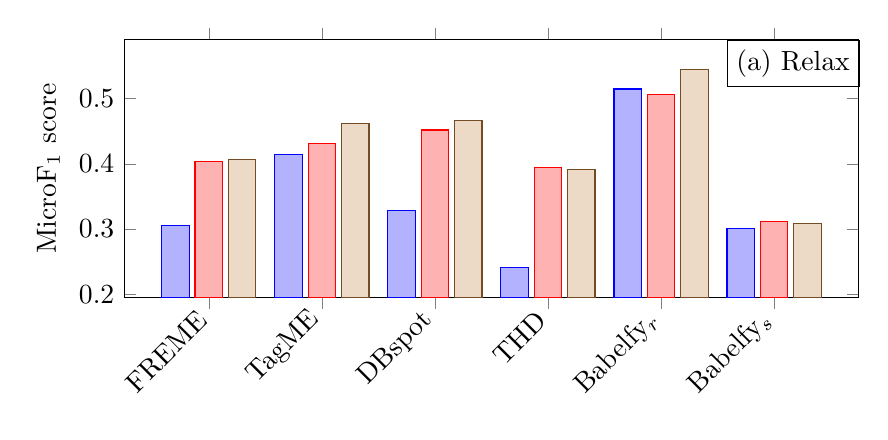
\begin{tikzpicture} 
\begin{axis}[ 
   title=(a) Relax,every axis title/.style={below right,at={(0.82,1)},draw=black,fill=white},
   ybar, 
   enlargelimits=0.15, 
   height=.4\textwidth,
   width=.9\textwidth,
   %legend style={at={(0.295,1)}, anchor=north,legend columns=-1}, 
   ylabel={MicroF$_1$ score}, 
   symbolic x coords={FREME,TagME,DBspot,THD, Babelfy$_r$,Babelfy$_s$}, 
   xtick=data, 
   %nodes near coords, 
   %nodes near coords align={vertical},
   x tick label style={rotate=45,anchor=east},
   %title=(relax)
 ] 
 \addplot coordinates {(FREME,0.306) (TagME,0.414) (DBspot,0.328) (THD,0.241) (Babelfy$_r$,0.515) (Babelfy$_s$,0.301)};
 \addplot coordinates {(FREME,0.404) (TagME,0.431) (DBspot,0.452) (THD,0.394) (Babelfy$_r$,0.507) (Babelfy$_s$,0.311)};
 \addplot coordinates {(FREME,0.407) (TagME,0.462) (DBspot,0.466) (THD,0.392) (Babelfy$_r$,0.545) (Babelfy$_s$,0.308)};
 %\legend{Calibrated,Translation,EN}
 \end{axis} 
\end{tikzpicture}


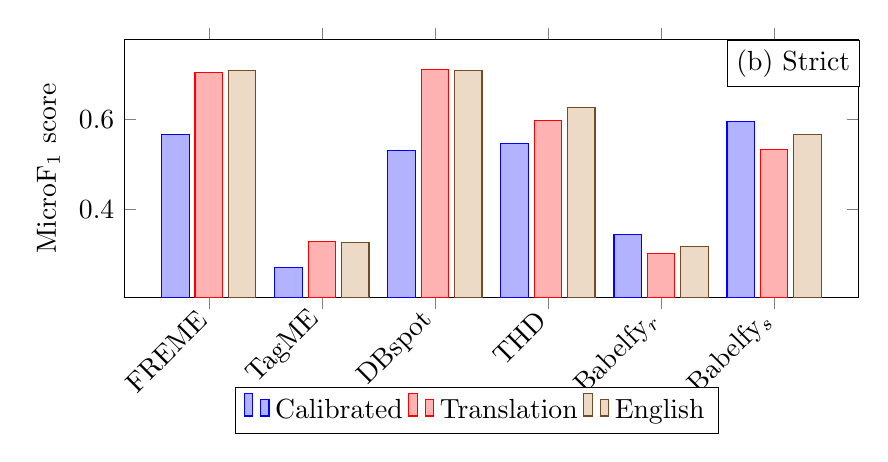
\begin{tikzpicture} 
\begin{axis}[ 
   title=(b) Strict,every axis title/.style={below right,at={(0.82,1)},draw=black,fill=white},
   ybar, 
   enlargelimits=0.15, 
   height=.4\textwidth,
   width=.9\textwidth,
   legend style={at={(0.48,-0.35)}, anchor=north,legend columns=-1}, 
   ylabel={MicroF$_1$ score}, 
   symbolic x coords={FREME,TagME,DBspot,THD, Babelfy$_r$,Babelfy$_s$}, 
   xtick=data, 
   %nodes near coords, 
   %nodes near coords align={vertical},
   x tick label style={rotate=45,anchor=east},
   %title=(relax)
 ] 
 \addplot coordinates {(FREME,0.567) (TagME,0.272) (DBspot,0.530) (THD,0.546) (Babelfy$_r$,0.345) (Babelfy$_s$,0.595)};
 \addplot coordinates {(FREME,0.704) (TagME,0.330) (DBspot,0.710) (THD,0.597) (Babelfy$_r$,0.302) (Babelfy$_s$,0.533)};
 \addplot coordinates {(FREME,0.708) (TagME,0.327) (DBspot,0.707) (THD,0.625) (Babelfy$_r$,0.319) (Babelfy$_s$,0.567)};
 \legend{Calibrated,Translation,English}
 \end{axis} 
\end{tikzpicture}
\end{figure}

%===============================================================
\section{Conclusion}
\label{sec:conclusion}

There are several multilingual approaches to address EL in the literature, as well as benchmark datasets that serve as a gold standard in the evaluation process. In this work we propose a manually annotated VoxEL, a new dataset that meets a set of properties that we consider desirable in multilingual EL assessments. Among these properties, we have that VoxEL has notes on cured texts, and not on texts translated automatically as is the case of some multilingual datasets of literature. This benefits to a greater extent to evaluate in a fair way the system that bases its models on intrinsic aspects of the lexicon. Also, we advocate for multilingual datasets that contain the same number of documents, sentences and annotations, in order to provide results that allow us the intra-language behavior of the systems. Property fulfilled by VoxEL.

We then conduct experiments to compare the performance of selected multilingual EL systems over VoxEL. We found an expected behavior in systems, being Babelfy and DBpedia Spotlight the best scored. In general, all the systems obtained better quality in the results for the annotations that only target persons, organizations and places. We also conducted experiments using VoxEL, to study how these systems perform when they are configured for the English language and an automatic translation is used to achieve multilingual annotation. 


{\footnotesize
\paragraph{Acknowledgements} The work of Henry Rosales-M\'endez was supported by CONICYT-PCHA/Doctorado Nacional/2016-21160017. The work was also supported by the Millennium Nucleus Center for Semantic Web Research under Grant NC120004. \textcolor{red}{We would like to thank Michael R\"oder for response some helpful email about GERBIL functionalities.}}

%
% ---- Bibliography ----
%
%\bibliographystyle{splncs}%splncs03}
%\bibliography{bibfile}

\bibliographystyle{splncs03}
\bibliography{bibfile}


%\begin{thebibliography}{99}
%%\bibitem{pdd2017electro_medical_kbs}
%%Wang, M., Zhang, J., Liu, J., Hu, W., Wang, S., Li, X., Liu, W. {PDD} {G}raph: {B}ridging Electronic Medical Records and Biomedical Knowledge Graphs via {E}ntity {L}inking. In ISWC, (2017)  219--227
%
%%\bibitem{UniProt2016kbbioinformatic}
%%UniProt Consortium. UniProt: the universal protein knowledgebase. Nucleic acids research, \textbf{45}(D1) (2016), D158--D169
%
%%\bibitem{flabase2015musickbs}
%%Oramas, S., Gómez, F., Gómez Gutiérrez, E., Mora, J. (2015). Flabase: Towards the creation of a flamenco music knowledge base. ISMIR (2015) 378--384
%
%\bibitem{Borrega2007}
%Borrega, O., Taul\'e, M., Mart\'i, M.A. What do we mean when we speak about Named Entities. In Proceedings of Corpus Linguistics, (2007)
%
%\bibitem{ourAMW2018}
%Rosales-M\'endez, H., Poblete, Barbara., Hogan, Aidan. What should Entity Linking link?. In AMW 2018
%
%\bibitem{Jha2017} 
%Jha, K., R\"oder, M., Ngomo, A. C. N. All that glitters is not gold–rule-based curation of reference datasets for named entity recognition and entity linking. In ESWC (2017) 305--320
%
%\bibitem{Babelfy-moro2014entity}
%Moro, A., Raganato, A., Navigli, R.: Entity linking meets word sense disambiguation: a unified approach. Trans. of the ACL \textbf{2} (2014) 231--244
%
%\bibitem{joinapproach2015}
%Gang Luo, Xiaojiang Huang, Chin-Yew Lin, and Zaiqing Nie. Joint named entity recognition and disambiguation. In Proc. EMNLP, 2015
%
%
%
%\bibitem{KIM-popov2004kim}
%Popov, B., Kiryakov, A., Ognyanoff, D., Manov, D., Kirilov, A.: KIM--a semantic platform for information extraction and retrieval. Natural Language Engineering \textbf{10}(3-4) (2004) 375--392
%
%\bibitem{SDA-charton2011automatic}
%Charton, E., Gagnon, M., Ozell, B.: Automatic semantic web annotation of named entities. In: Canadian Conference on Artificial Intelligence, Springer (2011) 74--85
%
%\bibitem{guo2012ualberta}
%Guo, Z., Xu, Y., de S{\'a} Mesquita, F., Barbosa, D., Kondrak, G.: ualberta at {TAC-KBP} 2012: English and cross-lingual entity linking. In: TAC. (2012)
%
%\bibitem{fahrni2012hits}
%Fahrni, A., G{\"o}ckel, T., Strube, M.: {HITS'} monolingual and cross-lingual entity linking system at {TAC} 2012: A joint approach. In: TAC, Citeseer (2012)
%
%\bibitem{THD-dojchinovski2012recognizing}
%Dojchinovski, M., Kliegr, T.: Recognizing, classifying and linking entities with {W}ikipedia and {DB}pedia. WIKT (2012) 41--44
%
%\bibitem{mendes2011dbpedia} 
%Mendes, P.N., Jakob, M., Garc{\'\i}a-Silva, A., Bizer, C.: {DB}pedia spotlight: shedding light on the web of documents. In: I-SEMANTICS, ACM (2011) 1--8
%
%\bibitem{daiber2013improving}
%Daiber, J., Jakob, M., Hokamp, C., Mendes, P.N.: Improving efficiency and accuracy in multilingual entity extraction. In: I-SEMANTICS, ACM (2013) 121--124
%
%\bibitem{ferragina2010tagme} 
%Ferragina, P., Scaiella, U.: Tagme: on-the-fly annotation of short text fragments (by Wikipedia entities). In: CIKM, ACM (2010) 1625--1628
%
%%\bibitem{narducci2013cross}
%%Narducci, F., Palmonari, M., Semeraro, G.: Cross-language semantic matching for discovering links to e-gov services in the {LOD C}loud. KNOW@ LOD \textbf{992} (2013) 21--32
%
%\bibitem{wang2013boosting}
%Wang, Z., Li, J., Tang, J.: Boosting cross-lingual knowledge linking via concept annotation. In: IJCAI. (2013) 2733--2739
%
%\bibitem{usbeck2014agdistis}
%Usbeck, R., Ngomo, A.C.N., R{\"o}der, M., Gerber, D., Coelho, S.A., Auer, S., Both, A.: {AGDISTIS}-graph-based disambiguation of named entities using linked data. In: ISWC, Springer (2014) 457--471
%
%\bibitem{Cross-Lingual-Wikifier-tsai2016cross}
%Tsai, C.T., Roth, D.: Cross-lingual wikification using multilingual embeddings. In: NAACL-HLT. (2016) 589--598
%
%\bibitem{FEL-pappu2017lightweight}
%Pappu, A., Blanco, R., Mehdad, Y., Stent, A., Thadani, K.: Lightweight multilingual entity extraction and linking. In: WSDM, ACM (2017) 365--374
%
%\bibitem{mag2017}
%Moussallem, D., Usbeck, R., R\"oeder, M., Ngomo, A. C. N. {MAG}: {A} Multilingual, Knowledge-base Agnostic and Deterministic Entity Linking Approach. {K-CAP} 2017 , ACM, (2017) 9:1--9:8
%
%\bibitem{fox2017}
%Speck, R., Ngomo, A. C. N. {E}nsemble Learning of Named Entity Recognition Algorithms using Multilayer Perceptron for the Multilingual Web of Data. In K-CAP, 2017
%
%\bibitem{freme-ner2016}
%Sasaki, F., Dojchinovski, M., Nehring, J. Chainable and Extendable Knowledge Integration Web Services. In ISWC, (2016) 89--101
%
%
%\bibitem{abstracts2016}
%Br\"ummer, M., Dojchinovski, M., Hellmann, S. DBpedia Abstracts: A Large-Scale, Open, Multilingual NLP Training Corpus. In LREC, (2016)
%
%\bibitem{aida2011}
%Hoffart, J., Yosef, M. A., Bordino, I., F\"urstenau, H., Pinkal, M., Spaniol, M., Taneva, B., Thater, S., Weikum, G. Robust disambiguation of named entities in text. In EMNLP (2011) 782--792
%
%\bibitem{kore50}
%Hoffart, J., Seufert, S., Nguyen, D. B., Theobald, M., Weikum, G. {KORE}: keyphrase overlap relatedness for entity disambiguation. In CIKM, 2012.
%
%\bibitem{IITB2009}
%Kulkarni, S., Singh, A., Ramakrishnan, G., Chakrabarti, S. Collective annotation of Wikipedia entities in web text. In SIGKDD, (2009) 457--466
%
%\bibitem{moro2015semeval} 
%Moro, A., Navigli, R.: {SemEval}-2015 {Task} 13: Multilingual all-words sense disambiguation and entity linking. In: SemEval@ NAACL-HLT. (2015) 288--297
%
%\bibitem{meantime2016}
%Minard, A. L., Speranza, M., Urizar, R., Altuna, B., van Erp, M. G. J., Schoen, A. M., van Son, C. M. MEANTIME, the NewsReader multilingual event and time corpus. In  2016
%
%\bibitem{MSNBC07}
%Cucerzan, S. Large-scale named entity disambiguation based on Wikipedia data. In EMNLP-CoNLL, 2007
%
%
%\bibitem{ace04}
%Ratinov, L., Roth, D., Downey, D., Anderson, M. Local and Global Algorithms for Disambiguation to Wikipedia. In Proceedings of the 49th Annual Meeting of the Association for Computational Linguistics: Human Language Technologies. ACL, (2011) 1375--1384
%
%\bibitem{ace04_old}
%Doddington, G. R., Mitchell, A., Przybocki, M. A., Ramshaw, L. A., Strassel, S., Weischedel, R. M. The Automatic Content Extraction (ACE) Program-Tasks, Data, and Evaluation. In LREC, 2 (2004)
%
%\bibitem{wes2015}
%Waitelonis, J., Exeler, C., Sack, H. Linked data enabled generalized vector space model to improve document retrieval. In NLP \& DBpedia 2015 workshop, 2015
%
%\bibitem{renden2016}  Brando, C., Frontini, F., and Ganascia, J. G. REDEN: Named Entity Linking in Digital Literary Editions Using Linked Data Sets. Complex Systems Informatics and Modeling Quarterly, (2016)\textbf{4}(7) 60--80
%
%
%\bibitem{n3}
%Röder, M., Usbeck, R., Hellmann, S., Gerber, D., Both, A. $N^3$-{A} Collection of Datasets for Named Entity Recognition and Disambiguation in the NLP Interchange Format. In LREC, (2014) 3529--3533
%
%\bibitem{aquaint}
%Milne, D.,Witten, I.H.: Learning to link with wikipedia. In CIKM, ACM (2008) 509--518
%
%\bibitem{nif2013}
%Hellmann, S., Lehmann, J., Auer, S., and Br\"ummer, M. Integrating NLP using linked data. In ISWC, (2013) 98–113
%
%\bibitem{gerbil2015}
%Usbeck, R. et al. GERBIL -- General Entity Annotation Benchmark Framework. In 24th WWW conference, 2015
%
%\bibitem{fu2010}
%B. Fu and R. Brennan. Cross-lingual ontology mapping and its use on the multilingual semantic web. In Proceedings of WWW Workshop on Multilingual Semantic Web, 2010.
%%%%%%%%%%%%%%%%%%%%%%%%%%%%%%%%%%%%%%%%%%%%%%%%%%%%%


%\begin{comment}
%\begin{table}[tb!]
%\centering
%\caption{My caption}
%\label{my-label}
%\begin{tabular}{@{}lcccccccccc@{}}
%\toprule
%            & \multicolumn{2}{c}{DE} & \multicolumn{2}{c}{EN} & \multicolumn{2}{c}{ES} & \multicolumn{2}{c}{FR} & \multicolumn{2}{c}{IT} \\ \midrule
%            %& Relax~~   & Strict    & Relax~~   & Strict    & Relax~~   & Strict    & Relax~~   & Strict    & Relax~~   & Strict    
%            &~~~$R$~~~  &~~~$S$~~~   &~~~$R$~~~  &~~~$S$~~~   &~~~$R$~~~  &~~~$S$~~~   &~~~$R$~~~  &~~~$S$~~~   &~~~$R$~~~  &~~~$S$~~~    
%            \\ \cmidrule(lr){2-3}\cmidrule(lr){4-5}\cmidrule(lr){6-7}\cmidrule(lr){8-9}\cmidrule(lr){10-11} 
%Babelfy$_r$ & 0.595   & 0.784   & 0.578   & 0.759  & 0.662  & 0.805   & 0.613   & 0.739  & 0.579   & 0.706        \\
%Babelfy$_s$ & 0.301   & 0.701   & 0.336   & 0.638  & 0.342  & 0.722   & 0.328   & 0.697  & 0.316   & 0.334        \\
%AGDISTIS    & 0.270   & 0.568   & 0.301   & 0.779  & 0.376  & 0.549   & 0.241   & 0.475  & 0.447   & 0.725        \\
%DBspot      & 0.600   & 0.641   & 0.650   & 0.706  & 0.506  & 0.492   & 0.466   & 0.512  & 0.569   & 0.651        \\
%FREME-NER   & 0.err   & err     & 0.508   & 0.550  & err    & err     & err     & err    & err     & err        \\
%Tagme 2     & 0.340   & 0.747   & 0.592   & 0.857  & -      & -       & -       & -      & 0.266   & 0.604        \\
%THD         & 0.194   & 0.500   & 0.386   & 0.719  & -      & -       & -       & -      & -       & -          \\ \bottomrule
%\end{tabular}
%\end{table}
%
%
%
%\begin{table}[tb!]
%\centering
%\caption{Otra version de la tabla anterior para quedarnos con la que mas nos acomode}
%\label{tab:gerbil}
%\begin{tabular}{@{}lccccccccccc@{}}
%%\begin{tabular}{@{}lllllllllll@{}}
%\toprule
%            & \multicolumn{5}{c}{Relax}   & \multicolumn{5}{c}{Strict}  \\ \midrule
%            &~~DE~~~&~~EN~~~&~~ES~~~&~~FR~~~&~~IT~~~&~~DE~~~&~~EN~~~&~~ES~~~&~~FR~~~&~~IT~~~\\
%            \cmidrule(lr){2-6}\cmidrule(lr){7-11}
%Babelfy$_r$ & 0.595  & 0.578 & 0.662 & 0.613 & 0.579 & 0.784 & 0.759 & 0.805 & 0.739 & 0.706 \\
%Babelfy$_s$ & 0.301  & 0.336 & 0.342 & 0.328 & 0.316 & 0.701 & 0.638 & 0.722 & 0.697 & 0.334 \\
%AGDISTIS    & 0.270  & 0.301 & 0.376 & 0.241 & 0.447 & 0.568 & 0.779 & 0.549 & 0.475 & 0.725 \\
%DBspot      & 0.600  & 0.650 & 0.506 & 0.466 & 0.569 & 0.641 & 0.706 & 0.492 & 0.512 & 0.651 \\
%FREME NER   & $err$  & 0.508 & $err$ & $err$ & $err$ & $err$ & 0.550 & $err$ & $err$ & $err$ \\
%Tagme 2     & 0.340  & 0.592 & -     & -     & 0.266 & 0.747 & 0.857 & -     & -     & 0.604 \\
%THD         & 0.194  & 0.386 & -     & -     & -     & 0.500 & 0.719 & -     & -     & -   \\ \bottomrule
%\end{tabular}
%\end{table}
%\end{comment}

%\end{thebibliography}

\end{document}
